\section{System Architecture}\label{sec:architecture}

\subsection{Hardware platform}\label{subsec:hw}

The system is a single host server with four AMD (Xilinx) Alveo U55C accelerator cards on PCIe Gen3 x16
(Table~\ref{tab:platform}). Each card carries the XCU55C device and 16~GiB of HBM2 organised as 32 pseudo channels
(PCs) of 512~MiB; every HBM AXI port of a kernel reaches any PC through the HBM switch~\cite{amd_ds978,amd_ug1393}.
Device capacities in Table~\ref{tab:platform} are those of the data sheet~\cite{amd_ds978}; utilisation, achieved
clock and PC bindings are taken from the post route reports of the bitstreams used here (Section~\ref{subsec:res-resources}).
The host has \NumHostCores~cores in \NumHostSockets~sockets and \NumHostRamGiB~GiB of memory; three cards are attached
to NUMA node~0 and one to node~1 (Section~\ref{subsec:res-host}).

\begin{table}[t]
\caption{Platform. Device values from the AMD U55C data sheet~\cite{amd_ds978}; host values captured by script at
measurement time (\texttt{results/hardware\_manifest.json}).}\label{tab:platform}
% generated by scripts/make_tables.py, do not edit
\begin{tabular}{@{}ll@{}}
\toprule
FPGA device & AMD XCU55C on Alveo U55C (4 cards, shell xilinx\_u55c\_gen3x16\_xdma\_base\_3) \\
HBM2 per card & 16 GiB in 32 pseudo channels of 512 MiB \\
Host CPU & 2 $\times$ AMD EPYC 7742 64-Core Processor, 128 cores, 256 threads \\
Host memory & 503 GiB \\
Card NUMA nodes & 01: 0, 21: 0, 41: 0, a1: 1 \\
OS, XRT, Vitis & Ubuntu 20.04.6 LTS (5.15.0-139-generic), XRT 2.16.204, Vitis 2023.2 \\
Python stack & Python 3.8.20, NumPy 1.24.4, Qiskit 1.2.4, Qiskit Aer 0.15.1 \\
\bottomrule
\end{tabular}

\end{table}

\subsection{Distribution of the statevector}\label{subsec:partition}

An $n$ qubit state of $2^n$ complex128 amplitudes (16~bytes each) is split into $S = C\,P$ \emph{slices} of $2^L$
amplitudes, $L = n - \log_2 S$, where $C \in \{1,2,4\}$ is the number of cards and $P$ the number of slices per card.
Physical qubits $0,\dots,L-1$ are local to a slice; the next $\log_2 P$ physical qubits select the slice inside a card
and the top $\log_2 C$ select the card. Card $j$ therefore holds every amplitude whose top $\log_2 C$ index bits
equal $j$, and each card divides its share into $P$ slices, each stored in one HBM buffer (Section~\ref{subsec:engine}). We call the
$\log_2 S$ qubits above $L$ the \emph{slice qubits}; the top $\log_2 C$ of them are the \emph{partition qubits}. Capacities follow directly: an $n$ qubit complex128 state needs $2^{n+4}$~bytes, i.e.\ 16~MiB at
$n=20$, 4~GiB at $n=28$, 8~GiB at $n=29$ and 16~GiB at $n=30$, so that four cards (64~GiB in total) can hold
up to $n = 31$ when the state uses all PCs (Section~\ref{subsec:res-maxwidth} explains why not $n=32$).

\subsection{Baseline design}\label{subsec:baseline-design}

The single card design of the companion paper~\cite{tiwari2026fpga30} uses sixteen HBM data ports in complex64. When the
datapath was widened to complex128 for this work, the sixteen port kernel no longer routed: the implementation failed
with routing congestion and no bitstream was produced. The data ports were therefore halved, which gives the baseline
kernel. Each data bank needs its own AXI port and the gate sequence one more, so the design could not simply
spread the state over all 32 PCs. The baseline design thus uses one compute unit per card with eight HBM data ports and one gate buffer port,
bound to HBM[0] to HBM[7] and HBM[8]; amplitude $i$ of a card's slice is stored in port $i \bmod 8$, so each card
addresses nine PCs (4.5~GiB) of its 16~GiB. The kernel implements the 19 opcodes of Table~\ref{tab:opcodes} in
complex128 arithmetic; gate angles are transferred as float32 and widened in the kernel. With $n_\ell = n - \log_2 C$
local qubits, a single qubit gate on local qubit $q$ visits the $2^{n_\ell-1}$ amplitude pairs
\begin{equation}
i_0 = \bigl((k \shr q) \shl (q+1)\bigr) \bor \bigl(k \band (2^q-1)\bigr), \qquad i_1 = i_0 + 2^q,
\qquad k = 0,\dots,2^{n_\ell-1}-1, \label{eq:pair}
\end{equation}
and applies the $2\times2$ gate matrix to $(\alpha_{i_0}, \alpha_{i_1})$. CX with control $c$ and target $t$ swaps
$\alpha_i$ and $\alpha_{i \oplus 2^t}$ for every $i$ with $(i \band 2^c) \ne 0$ and $(i \band 2^t) = 0$; CZ negates
\begin{equation}
\alpha_i \leftarrow -\alpha_i \quad \text{for every } i \text{ with } (i \band 2^c) \ne 0 \text{ and } (i \band 2^t) \ne 0.
\label{eq:cz}
\end{equation}
A controlled phase $\mathrm{CP}(\theta)$ whose control is partition bit $p_b$ of card index $j$ and whose target is
local qubit $q_t$ changes only amplitudes of the card itself:
\begin{equation}
\alpha_i' = \begin{cases} e^{i\theta}\,\alpha_i & \text{if } \bigl((j \shr p_b) \band 1\bigr) = 1 \text{ and }
\bigl((i \shr q_t) \band 1\bigr) = 1,\\ \alpha_i & \text{otherwise.}\end{cases} \label{eq:diag}
\end{equation}

\begin{table}[t]
\caption{Opcodes of the baseline kernel (19, complex128 arithmetic), as defined in its source.}\label{tab:opcodes}
\begin{tabular}{@{}rlrlrlrl@{}}
\toprule
Opcode & Gate & Opcode & Gate & Opcode & Gate & Opcode & Gate \\
\midrule
0 & I & 5 & $S$ & 10 & $\sqrt{X}^\dagger$ & 15 & $U_2(\phi,\lambda)$ \\
1 & $H$ & 6 & $T$ & 11 & $R_X(\theta)$ & 16 & $U_3(\theta,\phi,\lambda)$ \\
2 & $X$ & 7 & $S^\dagger$ & 12 & $R_Y(\theta)$ & 17 & CX \\
3 & $Y$ & 8 & $T^\dagger$ & 13 & $R_Z(\theta)$ & 18 & CZ \\
4 & $Z$ & 9 & $\sqrt{X}$ & 14 & $P(\phi)$ & & \\
\bottomrule
\end{tabular}
\end{table}
 A host process per card drives the kernel and takes part in a
three barrier exchange through shared host memory (Section~\ref{sec:host}). Its three routing paths are executed as
follows:
\begin{itemize}
\item \emph{Local gates} (all qubits below the partition qubits) are lowered to the 19 opcodes and executed by the
kernel on every card.
\item \emph{Diagonal gates on partition qubits} are executed on the host: each card reads its slice from HBM over
PCIe, multiplies it by the card dependent phase in NumPy and writes it back. No amplitudes cross between cards, but
each such gate moves the whole slice over PCIe twice.
\item \emph{Other gates on partition qubits} are executed on the host after the three barrier exchange: each card
reads its slice, publishes it to shared memory, computes its new slice from its partner slices in NumPy and writes it
back.
\end{itemize}
Hence the baseline design performs gate arithmetic on the host for every gate that touches a partition qubit.

\subsection{Engine}\label{subsec:engine}

The engine keeps the partition by the top qubits and the three gate classes of the baseline design, and
moves every gate that does not require amplitudes of another slice onto the FPGA. It reuses the MUX2 pass engine of the
companion single card simulator~\cite{tiwari2026fpga30}, widened to complex128 and extended by a per operation slice
enable.

\paragraph{One primitive.} Every gate is compiled into MUX2 records. A record $(t, c, M_0, M_1)$ applies the
$2\times 2$ complex128 matrix $M_1$ to the amplitude pairs $(i_0, i_0 \mathbin{|} 2^t)$ whose index has all bits of the
mask $c$ set, and $M_0$ to the others. A single qubit gate is $M_0 = M_1 = U$; a controlled $U$ is $M_0 = I$,
$M_1 = U$ with the controls in $c$; a two qubit diagonal gate with diagonal $(d_0,d_1,d_2,d_3)$ on qubits $(a,b)$ is one
record on $b$ with $c = 2^a$, $M_0 = \mathrm{diag}(d_0,d_2)$, $M_1 = \mathrm{diag}(d_1,d_3)$; any other two qubit gate
takes three records (cosine sine decomposition). Multi controlled gates (Toffoli, the Grover oracle) are a single
record. Matrices are stored as float64, so no gate parameter is rounded below double precision.

\paragraph{Slice enable.} Each record carries $(s_{\mathrm{mask}}, s_{\mathrm{val}}, s_{\mathrm{inv}})$; the
engine that holds the slice with logical index $s$ executes the record only if
$\bigl((s \mathbin{\&} s_{\mathrm{mask}}) = s_{\mathrm{val}}\bigr) \oplus s_{\mathrm{inv}}$. The slice index is a
kernel argument of every launch. This turns three classes of gates on slice qubits into local work:
\begin{enumerate}
\item[F1] \emph{Diagonal gates on slice qubits} ($Z$, $S$, $T$, $R_Z$, $P$, $CZ$, $CP$, $CR_Z$, $R_{ZZ}$ and any diagonal
gate) become scalar phase records under a slice enable; they move no data at all and run inside a pass that already
streams the slice.
\item[F2] \emph{Gates controlled by slice qubits} with a local target (for example $CX$ from a partition qubit to a
local qubit) run as ordinary records on the slices whose control bits are one.
\item[F3] \emph{$X$, $CX$ and Toffoli acting only on slice qubits} permute whole slices; they are implemented by
relabelling which buffer holds which logical slice, again without data movement. SWAP gates are always absorbed into
the logical to physical qubit map.
\end{enumerate}
Only non diagonal gates whose target is a slice qubit need amplitudes of other slices. For these the compiler swaps
the slice qubit with a local qubit (global to local remapping, as in distributed CPU and GPU
simulators~\cite{haner2017petabyte,deraedt2019massively,imamura2022mpiqulacs}) and keeps executing locally until the
local qubit is needed again. A remap exchanges half of each slice with its partner slice: between slices of the same
card it runs as a device copy kernel inside HBM; between cards the moving halves cross PCIe through host memory.
Each of F1 to F3 can be switched off, in which case the gate falls back to the remap path; Section~\ref{subsec:res-ablation}
uses these switches for the ablations.

\paragraph{Reach of every pseudo channel.} The engine avoids both limits of the baseline kernel. Each compute unit has a
single AXI port, and its instruction segment is stored in the same buffer as its slice, so no port is spent on
instructions; and the compute units, not the ports of one unit, provide the parallelism. The main build has
\NumEnginesFlagship~complex128 engines per card, each bound to \NumPcsPerEngineFlagship~PCs, so that the
\NumPcsUsedFlagship~PCs of each card hold the state (Section~\ref{subsec:res-resources}); with the four exchange units this
uses \NumHbmPortsFlagship~of the HBM port connections of the card. A build with sixteen complex128 engines (two PCs
each) placed but failed routing with conflicted nets inside the engines, the same congestion that limited the
baseline kernel; eight engines with four PCs each route at \NumClockFlagship~MHz and still reach every PC, which is
what matters for capacity. Engine count and memory reach are thus decoupled.

\paragraph{Pass engine.} Each compute unit (\NumEnginesFlagship~per card in the main build, each bound to
\NumPcsPerEngineFlagship~PCs) holds one slice while a slice fits one PC ($P = \NumEnginesFlagship$), and for the widest
states one slice per PC, which it processes in turn ($P = \NumPcsUsedFlagship$). It streams each slice through on chip tiles of $2^k$ amplitudes ($k \le 11$). A pass loads every tile once, applies all
records of the pass whose qubits lie in the tile window (up to four high qubits gathered per tile), and writes the
tile back, so a sequence of gates costs one read and one write of the slice instead of one per gate. Inside the
pass the compute stage updates two amplitude pairs per cycle at an initiation interval of one; the 512~bit HBM ports
move four amplitudes per cycle in each direction. All cards execute the same instruction segment concurrently; the
host starts every compute unit of every card and waits for all of them.

\begin{figure}[t]
\centering
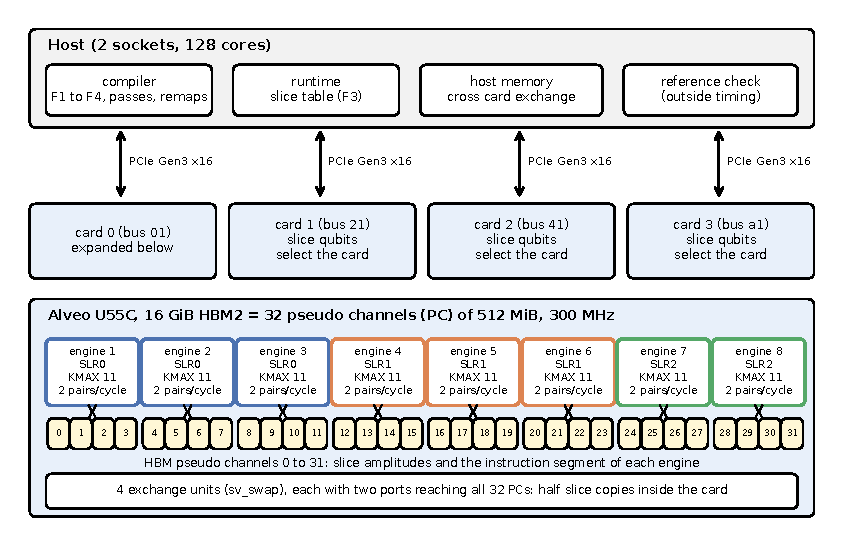
\includegraphics[width=\linewidth]{figures/fig_architecture.pdf}
\caption{Data flow of the engine on four cards. Local, slice controlled (F2) and slice diagonal (F1) gates
run in the HBM passes of every engine; slice relabelling (F3) changes only the slice table on the host; remaps
exchange half slices inside a card (device copy) or across cards (PCIe and host memory).}\label{fig:architecture}
\end{figure}
